%----------------------------------------------------------------------------------------
%	CHAPTER - LITERATURE REVIEW
%----------------------------------------------------------------------------------------

\chapter{Literature Review} % Main chapter title

\label{ChapterLiteratureReview} % Change X to a consecutive number; for referencing this chapter elsewhere, use \ref{ChapterX}

In the literature review chapter, an overview of existing research found in secondary literature, that is relevant to the thesis statement of this paper, is given. Every \gls{srq} is discussed in its own subchapter where its relevance to the \gls{mrq} is elaborated. Each subchapter ends with a short conclusion and answers to the corresponding research question are given.
Figure XXX shows the correlation between the subchapters and the research questions. In chapter \ref{SectionLiteratureReviewSRQ1}, the different methods for user input in virtual reality are analyzed. The next chapter \ref{SectionLiteratureReviewSRQ2} focuses on existing data interaction patterns in virtual reality. By looking at possible enhancements of existing interaction patterns with new methods for user input, the third SRQ is covered in chapter \ref{SectionLiteratureReviewSRQ3}. To wrap everything up, a conclusion of the literature review is presented in chapter \ref{SectionLiteratureReviewConclusion} which builds the base for the research design in chapter \ref{Research Method}.

% TODO: ADD FIGURE !!!


%----------------------------------------------------------------------------------------
%	SECTION 1
%----------------------------------------------------------------------------------------

\section{Different Methods for User Input in Virtual Reality}

\label{SectionLiteratureReviewSRQ1}

%-----------------------------------
%	SUBSECTION 1
%-----------------------------------
\subsection{Introduction}

\gls{hci} itself has been worked and research on approximately from the 1950s onwards, where the main focus was on the direct manipulation of graphical objects, the mouse as well as gesture recognition \citep{Myers1998}. During this time however, gesture recognition was rather understood as devices that work with pen-based input devices and thus can recognize patterns that are drawn with these pens \citep{Myers1998}. In the regular interactiion between human and machines this is still fairly sufficient as even today we are still fully relying on having a mouse/trackpad/touchscreen and a keyboard to interact with our computers. \newline
Virtual reality changes this since quite a bit as waering a \gls{hmd} with their own displays obstructs the view on the so far used physical input devices. New solutions had to be found for this changed situation. An overview on the researched interaction patterns with virtual reality is shown in the following subchapter.


%-----------------------------------
%	SUBSECTION 2
%-----------------------------------

\subsection{Overview}

The reviewed literature brought up different means in research to interact with the virtual reality environment. In order to review them in a more stuctured way, they have been grouped based on their core technology (i.e. hand gestures, speech recognition etc.) on which they base on. The regular game controllers have been excluded in this research since they basically are not much different from mouse and keyboard as they do not provide any added interaction functionality.


\subsubsection{Hand Gestures}

\label{SubSubSectionHandGestures}

The by far most utilized and researched interaction method is hand gestures. Since we also heavily rely on this interaction pattern in real life with other human beings, it is fair to assume that the familiarity of it helps the research in a significant way whereas methods that rely on physical hardware often feel more distant. \newline
\cite{Pfeiffer2008} conducted an empirical study about conversational pointing gestures in virtual reality interaction where the focus lied on the system to recognize on which object the user was pointing at. \cite{Pfeiffer2008} distinguished between \gls{ifp} where the direction of where the index finger is pointing at, and \gls{gfp} where an imaginary line between the viewers eye and the tip of the index finger is drawn. Provided the objects are nod too close to each other (>20cm), both methods had equal accuracy and success while tracked with two cameras from different angles and motion capturing \citep{Pfeiffer2008}. Figure \ref{fig:pointinggesture} shows the application of this in an identification game which was part of the empirical study.
\begin{figure}[h]
	\begin{center}
		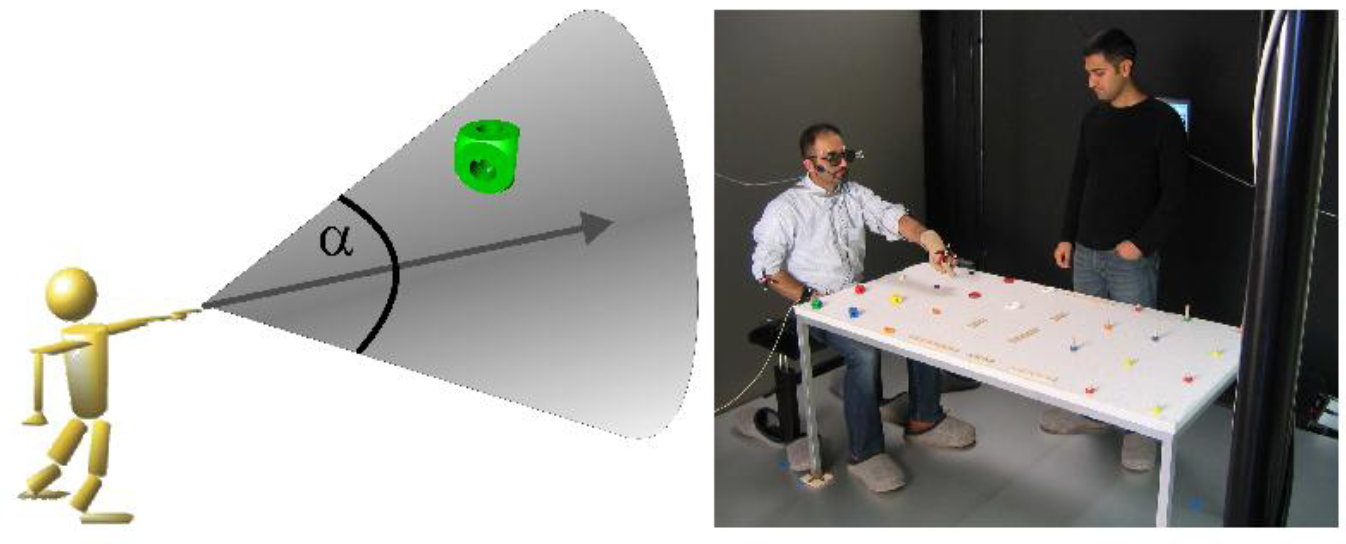
\includegraphics[width=10cm]{03_Figures/05_LitReview/Pfeiffer2008_Pointing.png}
		\caption[Cone-based model for extenstion of pointing gestures refined for identification game]{Cone-based model for extenstion of pointing gestures (left) refined for identification game (right) \citep{Pfeiffer2008}}
		\label{fig:pointinggesture}
	\end{center}
\end{figure}
\newline
A similar approach has been research by \cite{Rautaray2011} who used a single camera with an application that did the image capturing, locating the hand and its orientation and finally model the gesture to find a match for predefined gestures. The focus relied on simple gestures for \textit{punch} (three fingers), \textit{grab} (fist), \textit{throw} (five fingers), and to \textit{move forward} (thumb up) within a simple VR game \citep{Rautaray2011}. The recognition rate was between 80\% and 94\% (depending on the gesture), which might not be accurate enough for practical use cases as also acknowledged by \cite{Rautaray2011}. \newline
In a more recent study of \cite{Khundam2015}, it was not cameras that were used to track the hand gestures but a Leap Motion (an in-air controller) attached to the front of an Oculus Rift. Figure \ref{fig:leapmotion} shows the different gestures that were implemented by \cite{Khundam2015} in order to navigate within a virtual environment. Depending on how far the hand is moved towards a certain angle, the speed of the movement can be influenced to increase or decrease it \citep{Khundam2015}. Although the applied gestures are understandable and easy to learn, they still brings some unfamiliarity with them since in real life movement already has a specific gesture which however utilizes the legs and not the hands.
\begin{figure}[h]
	\begin{center}
		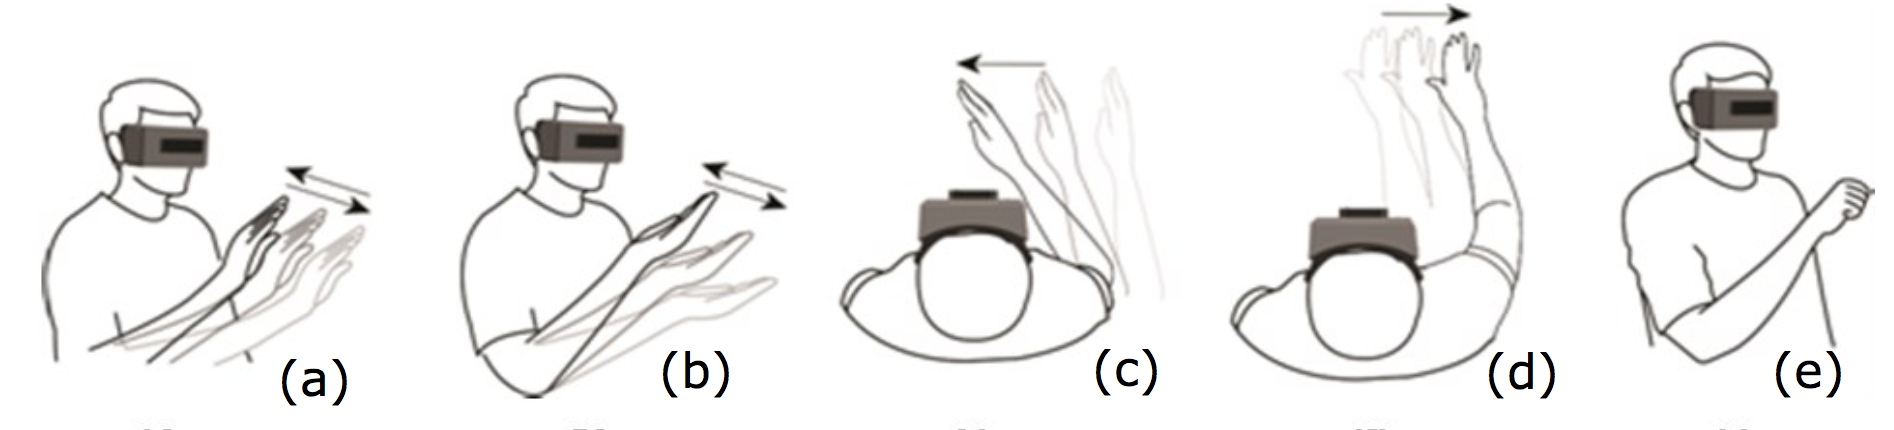
\includegraphics[width=14cm]{03_Figures/05_LitReview/Khundam2015_LeapMotion.png}
		\caption[Hand gestures for forward/backward movement, stepping left/right and holding position]{Hand gestures for forward/backward movement (a,b), stepping left/right (c,d) and holding position (e) \citep{Khundam2015}}
		\label{fig:leapmotion}
	\end{center}
\end{figure}
\newline
For their research on static and stroke gestures, \cite{Chun2015} made use of a depth-camera in order to track hand gestures and combined it with speech recognition. The latter is discussed in more detail in chapter \ref{SubSubSectionSpeechRecognition} which covers the methods of speech recognition in general. \cite{Chun2015} defined different hand and finger gestures for selecting, moving, scaling, rotating, copying and deleting objects, all of which actions had to be confirmed by a specific yes/no gesture. This set of gestures makes it a very natural, intuitive and interactive way for the user to alter virtual objects. As often with the use cameras, there are limitations to it. The hand has to be tracked properly for the whole performance of the gesture and it has to be done with the right speed for a proper recognition of the command \citep{Chun2015}.


\subsubsection{Gesture Controllers}

Very similar to the hand gestures, the gesture controllers intend to improve the tracking of the hand movements by adding hardware to the hands of the users that is easier to track but still leaves options for simple interaction with buttons and triggers. \newline
One of the first commercial gesture controllers was the \textit{PlayStation Move}, introduced by \cite{Sony2010}. While the controller itself can detect its own motion, the position is tracked with a camera attached to the PlayStation. This allows for a more accurate tracking of a specific point which \cite{Takala2014} made use of by attaching a PlayStation Miove to their HMD in order to have a more accurate positioning than it was possible with solely the Microsoft Kinect. \newline
Alongside the \textit{HTC Vive} HMD, a new gesture controller also have been introduced \citep{Htcvive2016}. In combination with the Lighthouse technology (described in chapter \ref{360MotionTracking}), the controllers can also be proberly tracked if they are e.g. hidden behind the back of the user, which is not possible with the PlayStation Move. Figure \ref{fig:gesturecontroller} shows this controller with its unique design for the tracking sensors (6) and a combination of trackpad (2), buttons (1, 3 and 8) and a trigger (7). By putting the thumb on the trackpad, the index finger on the trigger and the other three fingers on the side button it almost allows to track the grabbing motion of the hand.
\begin{figure}[h]
	\begin{center}
		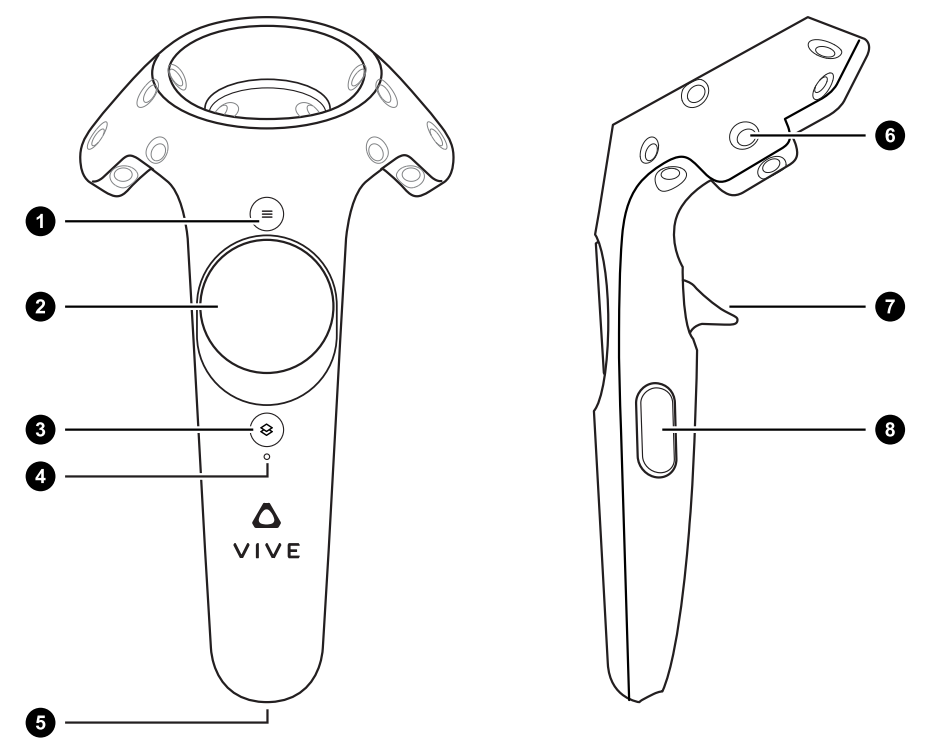
\includegraphics[width=10cm]{03_Figures/05_LitReview/HTCCorp2016_GestureController.png}
		\caption[Gesture Controller for the HTC Vive]{Gesture Controller for the HTC Vive \citep{HTCCorp2016}}
		\label{fig:gesturecontroller}
	\end{center}
\end{figure}


\subsubsection{Speech Recognition}

\label{SubSubSectionSpeechRecognition}

The second natural interaction after hand gestures is speech recongition. It is often combined with hand gesture as they can complement eachother quite seamlessly. \newline
For the navigation within 3D scans from \gls{mri} or \gls{ct}, \cite{Muller1998} proposed a speech recongition system as illustrated with an example in figure \ref{fig:speechrecognitionmedical}. With semantic decoding and a semantic strcuture, the commands can be interpreted and processed by the intention decoder to tell the system what to \citep{Muller1998}. This is a very time-consuming process since all commands have to be prepared and accoustic-phonetic models need to be generated during the collection of training data. Provided the users followed the instructions, a 99.8\% semantic accuracy could be acheived which basically means that the system is almost fully accurate in this scenario \citep{Muller1998}.
\begin{figure}[h]
	\begin{center}
		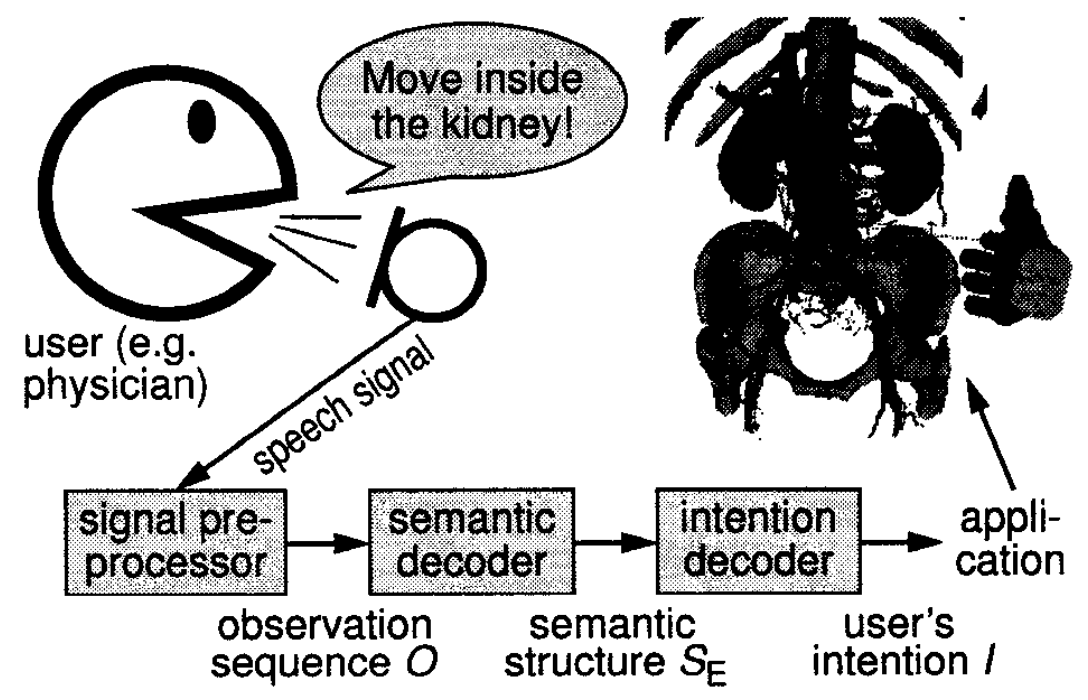
\includegraphics[width=10cm]{03_Figures/05_LitReview/Muller1998_SpeechRecognition.png}
		\caption[Architecture and example of speech recognition and interaction for physicians]{Architecture and example of speech recognition and interaction for physicians \citep{Muller1998}}
		\label{fig:speechrecognitionmedical}
	\end{center}
\end{figure}
\newline
\cite{Uchino2008} combined speech recognition with a camera to identify where the user is pointing at on a computer screen to interact with a virtual agent. In their example, a set of pens with different colours are presented to the user where the selection is made in combination with gestures (pointing at the pen) and speech (e.g. "\textit{Please give the red one}") \citep{Uchino2008}. Figure \ref{fig:speechrecignitionpen} shows how such a conversation with a virtual agent can proceed where the agent picks the wrong pen based on the pointing and ambiguous speech and thus has to be corrected to pick the one with the right color. Although this research was not focussed on virtual reality, this research can also be applied in virtual reality which might even improve the accurace of the pointing gesture.
\begin{figure}[h]
	\begin{center}
		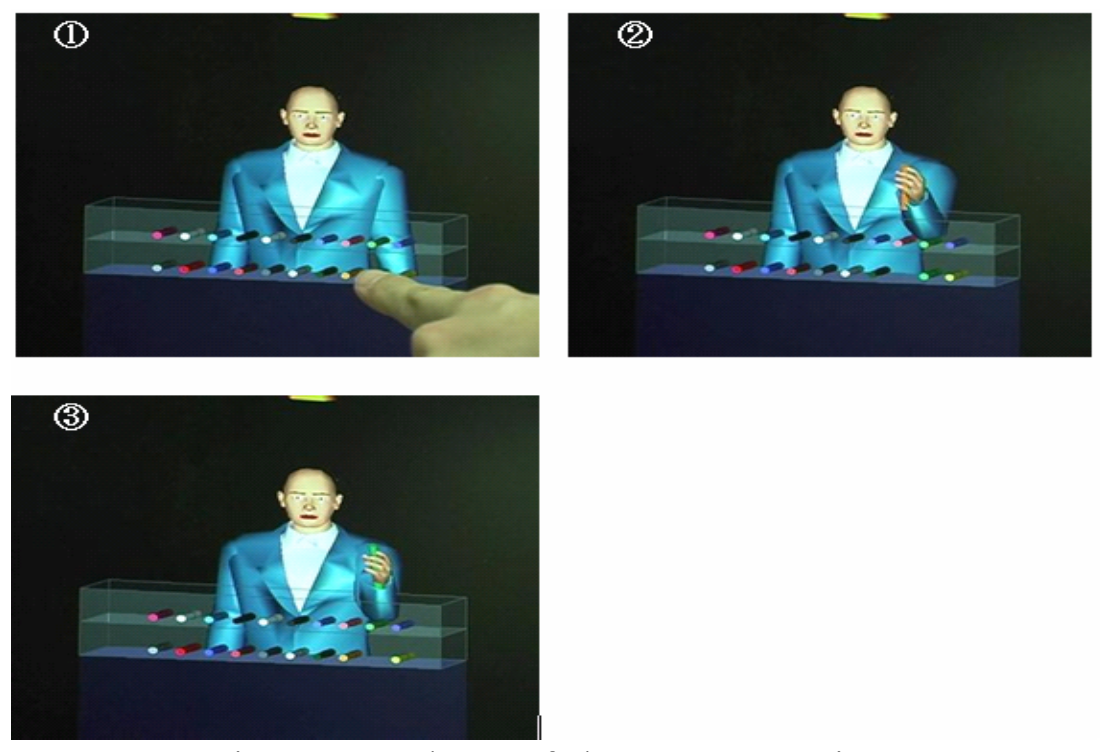
\includegraphics[width=10cm]{03_Figures/05_LitReview/Uchino2008_SpeechPointing.png}
		\caption[Flow of a conversation with the virtual pen agent]{Flow of a conversation with the virtual pen agent \citep{Uchino2008}}
		\label{fig:speechrecignitionpen}
	\end{center}
\end{figure}
\newline
As described in chapter \ref{SubSubSectionHandGestures}, \cite{Chun2015} utilized hand gestures to interact with virtual objects and further enhanced them with speech recognition. While objects can be altered in their spatial appearance, speech is used to change the colour of the object or ask questions about the type, shape or colour of it \citep{Chun2015}. Instead of relying on a physical device with buttons to change the colours, a multimodal interaction combines speech and gesture to a more natural and intuitive method that is also closer to the real world \citep{Chun2015} .


\subsubsection{Physical Placement of Interactive Objects}

Quite a bit older, from the 1990s, is the idea of dynamically placing physical knobs and switches in front of a seated user waring a HMD \citep{Latham1997}. The trajectory of the users hand and its movement is extrapolated in order to move the correct type of control in the right position just when it is expected in the virtual reality environment \citep{Latham1997}. Figure \ref{fig:touchcockpit} shows the concept of \cite{Latham1997} as well as how the final design looked like. Since such a machine requires a lot of time to design and build, it can be assumed that these are parts of the reason why not many further advancements were undertaken.
\begin{figure}[h]
	\begin{center}
		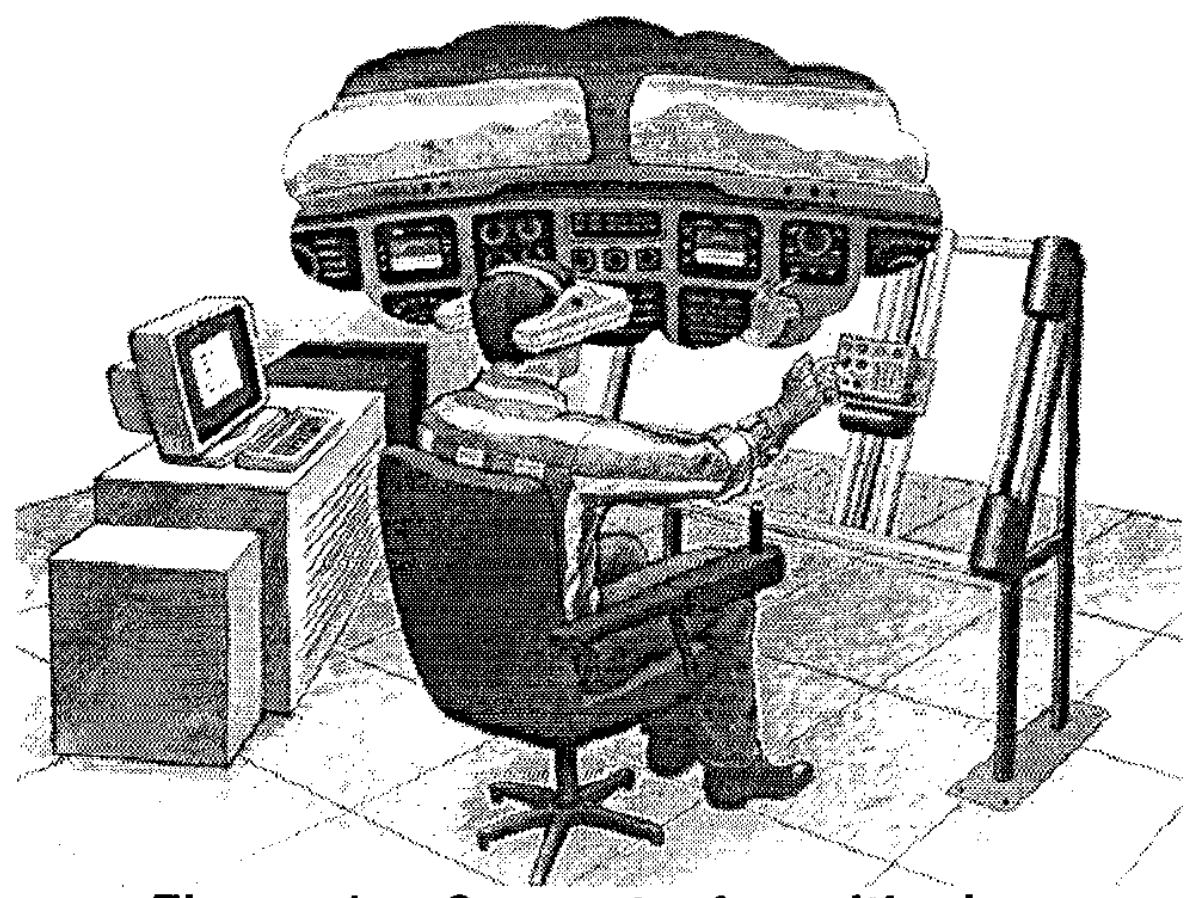
\includegraphics[width=6cm]{03_Figures/05_LitReview/Latham1997_Concept.png}
		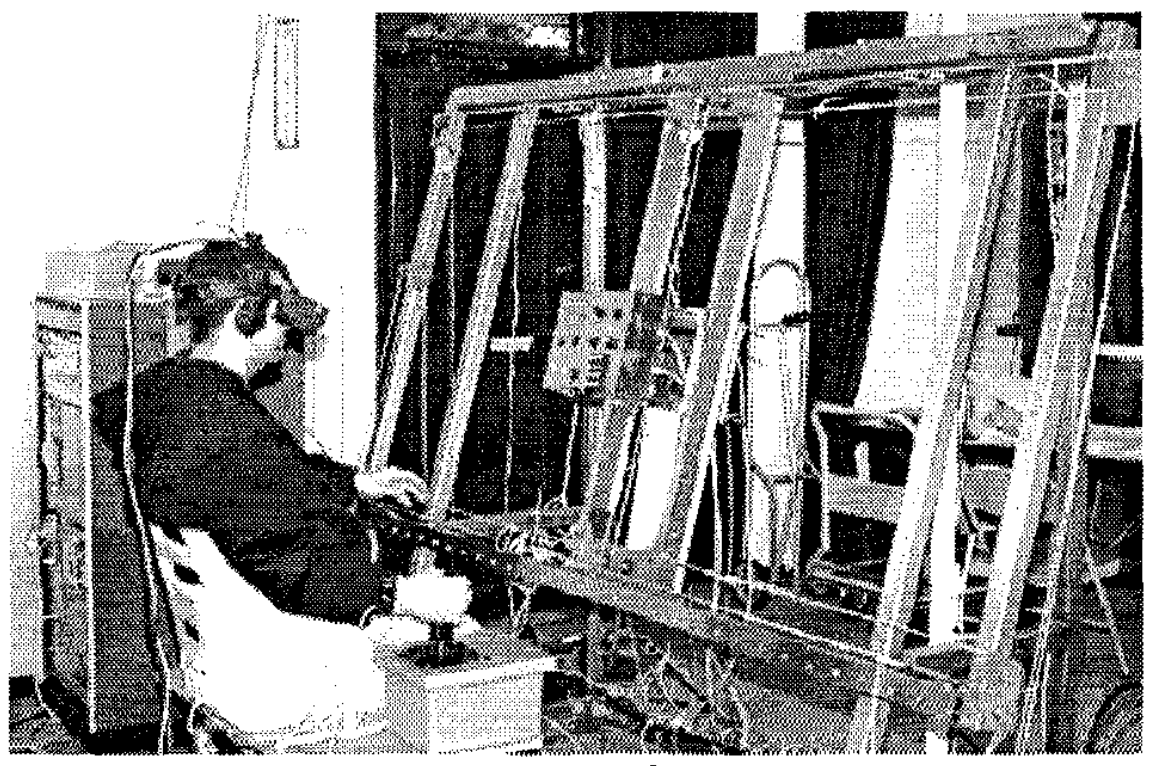
\includegraphics[width=7cm]{03_Figures/05_LitReview/Latham1997_FinalDesign.png}
		\caption[Concept and final design of positioning instrument controls to be touched in a virtual cockpit]{Concept (left) and final design (right) of positioning instrument controls to be touched in a virtual cockpit \citep{Latham1997}}
		\label{fig:touchcockpit}
	\end{center}
\end{figure}


\subsubsection{Full Body Tracking}

In June 2010, Microsoft announced the \textit{Kinect for Xbox 360}, a controller-free gaming device for the living room \citep{Microsoft2010}. Instead of relying on any physical input devices, the Kinect contains a comarea with motion-sensing technology that can track up to 48 points of movement on the human body, turning the player himself into a controller \citep{Microsoft2010}. \newline
Based on this technology, \cite{Takala2014} proposed a combination of a full body avatar controlled by Kinect with the Oculus Rift as display. This combination proved to be quite powerfull although they were facing a couple of challenges as well. The Kinect sometimes lost track of the hands or the movement was not recognized at all which \cite{Takala2014} tried to resolve by attaching a PlayStation Move to the HMD and put a Razer Hydra controller into the hands (Figure \ref{fig:kinectbody}). Although this improved the situation, different latencies of the individual dampened the experience. Furthermore, although Kinect was used for full-body tracking, only the movement of the hands and legs was utilized, whereas the movement within the virtual world was still relying on a physical controller.
\begin{figure}[h]
	\begin{center}
		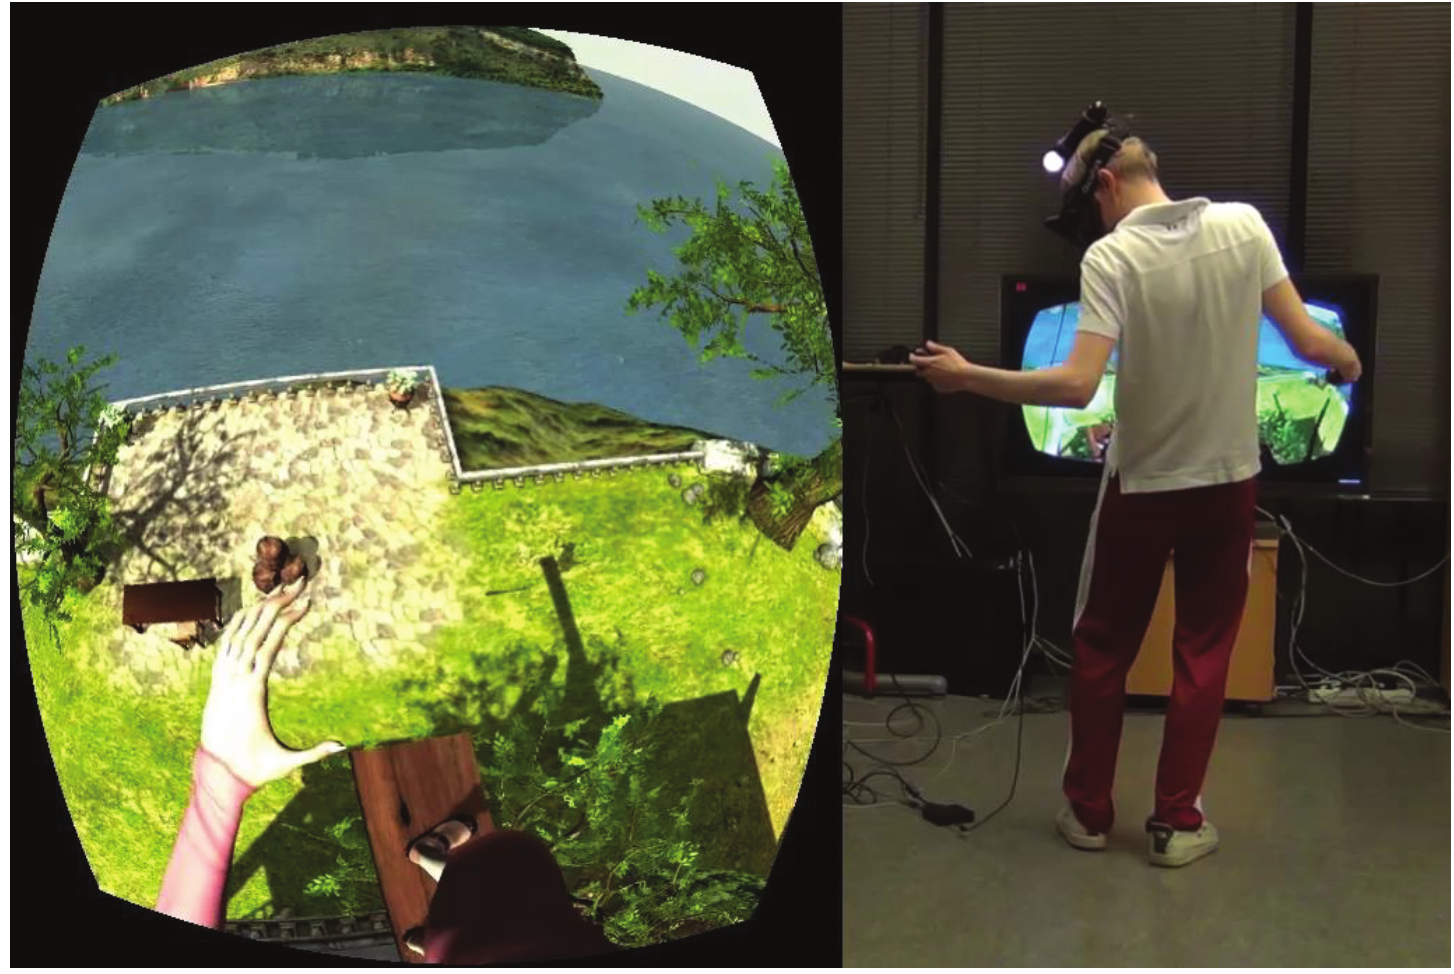
\includegraphics[width=12cm]{03_Figures/05_LitReview/Takala2014_KinectBody.png}
		\caption[Player's view of their virtual body that is tracked with Kinect]{Player's view of their virtual body (left) that is tracked with Kinect (right) \citep{Takala2014}}
		\label{fig:kinectbody}
	\end{center}
\end{figure}


\subsubsection{360° Motion Tracking}
\label{360MotionTracking}

One of the latest additions to the interaction possibilities is the 360° motion tracking, introduced with the HTC Vive which was just released in April 2016 \citep{Htcvive2016}. Figure \ref{fig:lighthouses} shows the setup of the two base stations (i.e. Lightouses) in opposing corners of the room that will be used for the 360° motion tracking. In essence, the two Lighthouse base stations emit a laser sweap across the room 60 times a second with a flash in between which allows any device with photosensors to calculate its exact position relative to the base station(s) \citep{Gizmodo2015}. This allows for a very accurate tracking and due to the opposing corners, at least one Lighthouse always has direct \textit{line of sight} to the HMD and the controllers. \newline
With this additional sensor information, the movement of the HMD and the controllers is tracked in all three axis and allow for new movements to be recognized, such as crouching or jumping within the relations of the room. \newline
So far there are no official devices that track the position of the feet, though this might only be a question of time.
\begin{figure}[h]
	\begin{center}
		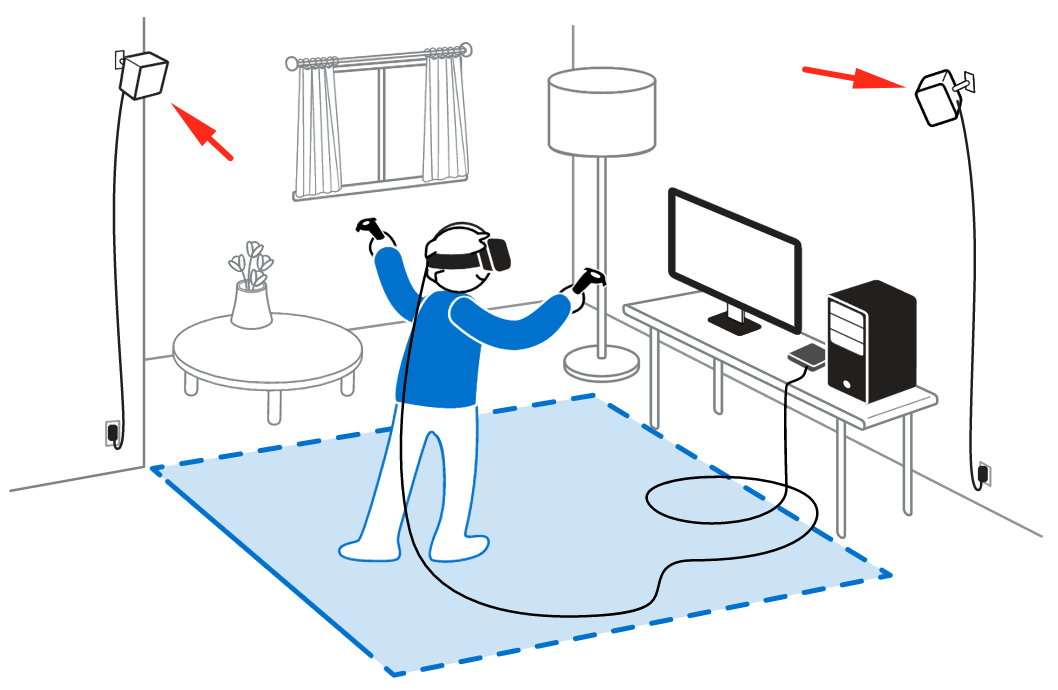
\includegraphics[width=10cm]{03_Figures/05_LitReview/HTCCorp2016_LighthouseRoomScale.png}
		\caption[Two Lighthouse in opposing corners allow for 360° motion tracking]{Two Lighthouse in opposing corners allow for 360° motion tracking \citep{HTCCorp2016}}
		\label{fig:lighthouses}
	\end{center}
\end{figure}


%-----------------------------------
%	SUBSECTION 3
%-----------------------------------

\subsection{Conclusion}

The literature review on different methods for user input in virtual reality showed that there are various types can be used or even combined. \newline
There are six main methods for user input in virtual reality. These are hand gestures, gesture controllers, speech recognition, physical placement of interactive objects, full body tracking and 360° motion tracking. Hand gestures track the movement of the whole hand and/or the individual fingers with one or more (regular, infrared or depth) cameras. Gesture controllers are physical devices with buttons that are held in the hands and also tracked in their spatial position. Speech recognition tries to understand and interpret spoken words and sentences in order to find the correct commands. The physical placement of interatice objects extrapolates the movement of the hand to physically place a button in front of the finger where a virtual one is shown in VR. Full body tracking uses cameras to track the whole body including the movement of all extremities from one angle. Finally, 360° motion tracking can locate the position of special devices within an actual room on all three axis from opposing corners. The most used method in the reviewed literature is the hand gestures, followed by the hand gestures in combination with speech recongition. \newline
Depending on the method, there are advantages and disadvantages (or even limitations) for certain use cases. Table \ref{tbl:methodscomparison} shows a summary of these findings.

\begin{table}[h!]
	\begin{center}
		\begin{tabular}{ | p{3.7cm} | p{4.9cm} | p{4.9cm} | } 
			\hline
			\textbf{Method} & \textbf{Advantages} & \textbf{Disadvantages} \\
			\hline
				Hand Gestures & 
				- Highest familiarity \newline - Inexpensive & 
				- Limited tracking area \newline - Only from one angle \newline - Decreasing accuracy with faster movement  \\
			\hline
				Gesture Controllers &
				- Very accurate \newline - Hand-held device (similarity to hand gestures) \newline - Buttons for more interaction &
				- Additional device required \newline - Have to be held all the time \\
			\hline
				Speech Recognition &
				- Most natural to humans \newline - Known from smartphones &
				- Different languages, dialects \newline - Requires silent area \\ 
			\hline
				Physical Placement of Objects &
				- Realistic experience \newline Tangible interaction with VR &
				- Expensive \newline - Difficult to build \newline - Stationary \\ 
			\hline
				Full Body Tracking &
				- Tracks all extremities \newline - Natural interaction possible &
				- Only from one angle \newline - Limited accuracy on details \\ 
			\hline
				360° Motion Tracking &
				- Room-scale tracking \newline - Very accurate \newline - Spatial positioning on all three axis &
				- Only HMD and controllers are tracked \newline - Expensive \\ 
			\hline
		\end{tabular}
		\caption{Advantages and disadvantages/limitations of different methods for user input in virtual reality}
		\label{tbl:methodscomparison}
	\end{center}
\end{table}


Hand Gestures = Limited tracking area (in front of camera etc attached to HMD), mostly accurate, most familiar to us, one angle only
Gesture Controllers = Accuracy, input is directly in the ands, couple of buttons etc to interact, tangible, hand gstures used for movement (irritating)
Speech Recongition = Hard to interpret correctly (Siri etc.), language, dialect, ...
Physical Placement = Expensive, difficutl to build, stationary, 
Full Body Tracking = One angle, all extremities covered however, not very accurate
Motion Tracking = Room-scale, multi-angle, only HMD and controller covered, very accurate


%----------------------------------------------------------------------------------------
%	SECTION 2
%----------------------------------------------------------------------------------------

\section{Existing Data Interaction Patterns in Virtual Reality}

\label{SectionLiteratureReviewSRQ2}

%-----------------------------------
%	SUBSECTION 1
%-----------------------------------

\subsection{Introduction}

blub


TO CHECK: “Put-that-there”: Voice and Gesture at the Graphics Interface \citep{Bolt1980}

TO CHECK: ALl interaction in RL is multimodal \cite{Bunt1998}

%-----------------------------------
%	SUBSECTION 2
%-----------------------------------

\subsection{Visual Information Seeking Mantra}

blub

%-----------------------------------
%	SUBSECTION 3
%-----------------------------------

\subsection{Conclusion}

blub



%----------------------------------------------------------------------------------------
%	SECTION 3
%----------------------------------------------------------------------------------------

\section{Enhancement of Existing Interaction Patterns with new Methods for User Input}

\label{SectionLiteratureReviewSRQ3}

%-----------------------------------
%	SUBSECTION 1
%-----------------------------------

\subsection{Introduction}

blub


%-----------------------------------
%	SUBSECTION 2
%-----------------------------------

\subsection{tbd}

blub

%-----------------------------------
%	SUBSECTION 3
%-----------------------------------

\subsection{Conclusion}

blub




%----------------------------------------------------------------------------------------
%	SECTION 4
%----------------------------------------------------------------------------------------

\section{Conclusion}

\label{SectionLiteratureReviewConclusion}

blub

